\chapter{Results}\label{chap:results}

The main goal of this analysis was to quantify key metrics of the performance of LGAD sensors. In particular, we analyzed the collected charge, the time resolution and the efficiency at the temperature of \qty{-30}{\degreeCelsius}, which will be the temperature of the detector in operation. We compared the results between unirradiated and differently irradiated sensors to test whether the requirements at start and end of life were satisfied. The sensors were also studied at angles between \qty{0}{\degree} and \qty{14}{\degree} relative to the beam direction, in line with the HGTD's expected pseudorapidity coverage: between \(2.4\) and \(4\), which corresponds to incident angles of \qtyrange{2}{10}{\degree}.

Additionally, some other properties and effects that arose during the analysis were also investigated. Such as, signal coming from neighbouring pads, noise coming from outside the gain layer of the pads, and properties of the region lying between two adjacent pads. Certain anomalies were also successfully explained, and the root cause was found in the incorrect voltage range set on an oscilloscope, which caused pulses to be "clipped" below a specific threshold. Moreover, due to a temporary malfunction of the cooling box, one batch of data showed neatly the sensitivity of LGADs to temperature variations.

\section{Main Results}

\begin{figure}[h!tbp]
    \centering
    \includegraphics[width=.9\linewidth]{Images/Results/Irradiated/IME_voltage_charge_.png}
    \captionsetup{width=\captionwidth}
    \caption{Overview of voltage vs collected charge for all the studied sensors from IME. \(\Phi\) is the radiation dose of each sensor in neutron-equivalent fluence.}
    \label{fig:irradiated_IME_voltage_charge}
\end{figure}


\begin{figure}[h!tbp]
    \centering
    \includegraphics[width=.9\linewidth]{Images/Results/Irradiated/IME_voltage_time_resolution_.png}
    \captionsetup{width=\captionwidth}
    \caption{Overview of voltage vs time resolution.}
    \label{fig:irradiated_IME_voltage_time_res}
\end{figure}

The most important properties of the sensors are:

\begin{itemize}
    \item Collected change: the most probable value (MPV) of the Landau*Gaussian convolution (Section~\ref{sec:methods_collected_charge}).
    \item Time resolution: the spread of the Gaussian distribution of the Time of Arrivals (Section~\ref{sec:methods_time_resolution}).
    \item Efficiency: the fraction of incident particles that produce a detectable signal in the sensor. (Section~\ref{sec:methods_efficiency}).
\end{itemize}

Overall all sensors behaved as expected: their collected charge increased with higher bias voltage and decreased with higher radiation dose (fluence), and most of them satisfied the HGTD's requirements.

\subsection{Irradiated samples performance}

\subsubsection{IME}

The sensors in the IME group were further split depending on versions and types, to enable more meaningful comparisons between devices with similar characteristics. More specifically:

\begin{itemize}
    \item IMEv3-W12: 2\(\times\)2 array unirradiated, 1\(\times\)3 array unirradiated and 2\(\times\)2 array at \qty{1.5e15}{\neutroneq}.
    \item IMEv2-W7: single pad at \qty{1e14}{\neutroneq} and single pad at \qty{6.5e14}{\neutroneq}.
    \item IMEv3-W16: single pad at \qty{8e14}{\neutroneq} and single pad at \qty{2.5e15}{\neutroneq}.
\end{itemize}

%%% IMEv3-W12, 0 and 
\begin{figure}[h!tbp]
    \centering
    \subfloat[Voltage vs Charge.]{
        \includegraphics[width=.49\linewidth]{Images/Results/Irradiated/IMEv3-W12_voltage_charge_irradiated.png}
        \label{fig:IMEv3-W12_voltage_charge}}
    \hfill
    \subfloat[Voltage vs Time resolution]{
        \includegraphics[width=.47\linewidth]{Images/Results/Irradiated/IMEv3-W12_voltage_time_resolution_irradiated.png}
        \label{fig:IMEv3-W12_voltage_time_res}}
    \vfill
    \subfloat[Voltage vs Efficiency]{
        \includegraphics[width=.47\linewidth]{Images/Results/Irradiated/IMEv3-W12_voltage_efficiency_irradiated.png}
        \label{fig:IMEv3-W12_voltage_efficiency}}
    \captionsetup{width=\captionwidth}
    \caption{IMEv3-W12. The non irradiated sensors (both the 2\(\times\)2 array and the 1\(\times\)3 array) had sufficiently high collected charge at all tested bias voltages, while the time resolution was just short of the \qty{35}{\pico\second} target in the case of the 2\(\times\)2 array, although this is likely to be solved with higher applied voltage. The lack of data for higher voltages was due to erroneous batches. It should be noted that the two pads of the 1\(\times\)3 array had significant and consistent discrepancies in charge and time resolution, presumably due to differences at the manufacturing stage. The sensors at \qty{1.5e15}{\neutroneq} had very good performance overall and still reached the target time resolution of beginning of operations (\qty{35}{\pico\second}) at \(\simeq60\%\) of the total expected dose. The efficiency satisfied the \(95\%\) goal above \(\approx\qty{400}{\volt}\).}
\end{figure}

\begin{figure}[p!htb]
    \centering
    \subfloat[Voltage vs Charge]{
        \includegraphics[width=.47\linewidth]{Images/Results/Irradiated/IMEv2-W7_voltage_charge_irradiated.png}
        \label{fig:IMEv2-W7_voltage_charge}}
    \hfill
    \subfloat[Voltage vs Time resolution]{
        \includegraphics[width=.45\linewidth]{Images/Results/Irradiated/IMEv2-W7_voltage_time_resolution_irradiated.png}
        \label{fig:IMEv2-W7_voltage_time_res}}
    \vfill
    \begin{minipage}[c]{.47\linewidth}
    \subfloat[Voltage vs Efficiency]{
        \includegraphics[width=.95\linewidth]{Images/Results/Irradiated/IMEv2-W7_voltage_efficiency_irradiated.png}
        \label{fig:IMEv2-W7_voltage_efficiency}}
        % \captionsetup{width=\captionwidth}
    \end{minipage}
    \hfill
    \begin{minipage}[c]{.5\linewidth}
        \captionof{figure}{IMEv2-W7. For both fluences (\qty{1e14}{\neutroneq} and \qty{6.5e14}{\neutroneq}, i.e. low fluence) charge, time resolution and efficiency were within the targets for larger voltages. Although, the more heavily irradiated sensor showed a significant variation in the efficiency, which increased from \(\approx30\%\) up to \(\approx95\%\).}
\end{minipage}
\end{figure}

\begin{figure}[p!htb]
    \centering
    \subfloat[Voltage vs Charge]{
        \includegraphics[width=.47\linewidth]{Images/Results/Irradiated/IMEv3-W16_voltage_charge_irradiated.png}
        \label{fig:IMEv3-W16_voltage_charge}}
    \hfill
    \subfloat[Voltage vs Time resolution]{
        \includegraphics[width=.45\linewidth]{Images/Results/Irradiated/IMEv3-W16_voltage_time_resolution_irradiated.png}
        \label{figIMEv3-W16_voltage_time_res}}
    \vfill
    \begin{minipage}[c]{.47\linewidth}
    \subfloat[Voltage vs Efficiency]{
        \includegraphics[width=.95\linewidth]{Images/Results/Irradiated/IMEv3-W16_voltage_efficiency_irradiated.png}
        \label{fig:IMEv3-W16_voltage_efficiency}}
    \end{minipage}
    \hfill
    \begin{minipage}[c]{.5\linewidth}
    \captionof{figure}{IMEv3-W16. The sensor at \qty{8e14}{\neutroneq} performed well overall, except for the batch at highest bias voltage, which saw a small but unexpected worsening of time resolution and efficiency. We investigated it further, but we were unable to pinpoint the exact cause. The sensor at \qty{2.5e15}{\neutroneq}, corresponding to the end-of-life radiation dose, had a collected charge below the requirements, slightly below \qty{3}{\femto\coulomb} and very poor efficiency, but it showed satisfactory time resolution.}
\end{minipage}
\end{figure}

\FloatBarrier

\subsubsection{USTC}

The data from the USTC sensor was the most affected by missing and erroneous batches, as the data from the irradiated sensor was not available.

\begin{figure}[h!tbp]
    \centering
    \subfloat[Voltage vs Charge]{
        \includegraphics[width=.47\linewidth]{Images/Results/Irradiated/USTC_voltage_charge_.png}
        \label{fig:USTC_voltage_charge}}
    \hfill
    \subfloat[Voltage vs Time resolution]{
        \includegraphics[width=.45\linewidth]{Images/Results/Irradiated/USTC_voltage_time_resolution_.png}
        \label{fig:USTC_voltage_time_res}}
    \vfill
    \begin{minipage}[c]{.47\linewidth}
    \subfloat[Voltage vs Efficiency]{
        \includegraphics[width=.95\linewidth]{Images/Results/Irradiated/USTC_voltage_efficiency_.png}
        \label{fig:USTC_voltage_efficiency}}
    \end{minipage}
    \hfill
    \begin{minipage}[c]{.5\linewidth}
        \captionof{figure}{USTC. The sensor had very good collected charge and efficiency, albeit falling short of the time resolution aim. It also manifested evident differences between the two neighbouring pads. Unfortunately, the data of the irradiated USTC sensor was not available, so no comparison was possible.}
\end{minipage}
\end{figure}

\subsubsection{CNM}

The unirradiated sensors were used to measure the time resolution of the MCP (Section~\ref{sec:MCP_description}). They had already been tested before (as in \cite{Allaire:2018bof}) and they showed similar performance, with gain up to \qtyrange{40}{50}{}, and time resolution better than \qty{30}{\pico\second}. In this test beam they were also tested irradiated at two fluences: \qty{1.5e15}{\neutroneq} and \qty{2.5e15}{\neutroneq}.

\begin{figure}[h!tbp]
    \centering
    \subfloat[Voltage vs Charge]{
        \includegraphics[width=.47\linewidth]{Images/Results/Irradiated/CNM_voltage_charge_.png}
        \label{fig:CNM_voltage_charge}}
    \hfill
    \subfloat[Voltage vs Time resolution]{
        \includegraphics[width=.45\linewidth]{Images/Results/Irradiated/CNM_voltage_time_resolution_.png}
        \label{fig:CNM_voltage_time_res}}
    \vfill
    \begin{minipage}[c]{.47\linewidth}
    \subfloat[Voltage vs Efficiency]{
        \includegraphics[width=.95\linewidth]{Images/Results/Irradiated/CNM_voltage_efficiency_.png}
        \label{fig:CNM_voltage_efficiency}}
    \end{minipage}
    \hfill
    \begin{minipage}[c]{.5\linewidth}
        \captionof{figure}{CNM. The good performance of the unirradiated sensors was confirmed. At the highest expected radiation dose the sensor had an unexpected counter trend of time resolution, however, the two batches at lower voltages had a significantly lower amount of data available, potentially underestimating the error on the fit. Also, the efficiency (with a threshold of \qty{4}{\femto\coulomb}) did not reach \(30\%\) even at \qty{600}{\volt}.}
\end{minipage}
\end{figure}

\FloatBarrier 

\subsection{Angled samples performance}

When particles traverse a sensor at an angle, the effective path inside the volume of the sensor will be slightly longer (\(\approx3\%\) at \qty{14}{\degree}). For this reason, charge deposition will be greater and a small improvement in the performance is expected.
The sensors were studied with incident angles of \qty{0}{\degree}, \qty{6}{\degree} and \qty{14}{\degree}. However, due to some missing or erroneous batches or mismatched voltages and angles, not all data points were available.

\subsubsection{IME}

%%% IMEv3-W12 2x2 100V
\begin{figure}[h!tbp]
    \centering
    \subfloat[Angle vs Charge]{
        \includegraphics[width=.47\linewidth]{Images/Results/angled/IMEv3-W12_angle_charge_-100V.png}
        \label{fig:IMEv3-W12_angle_charge_100V}}
    \hfill
    \subfloat[Angle vs Time resolution]{
        \includegraphics[width=.45\linewidth]{Images/Results/angled/IMEv3-W12_angle_time_resolution_-100V.png}
        \label{fig:IMEv3-W12_angle_time_res_100V}}
    \vfill
    \begin{minipage}[c]{.47\linewidth}
        \subfloat[Angle vs Efficiency]{
            \includegraphics[width=.95\linewidth]{Images/Results/angled/IMEv3-W12_angle_efficiency_-100V.png}
            \label{fig:IMEv3-W12_angle_efficiency_100V}}
    \end{minipage}
    \hfill
    \begin{minipage}[c]{.5\linewidth}
        \captionof{figure}{IMEv3-W12, 2\(\times\)2 array, at \qty{-100}{\volt}. The impact of the angle was small, although it showed an improvement in collected charge and time resolution, as expected.}
\end{minipage}

\end{figure}

%%% IMEv3-W12 1x3 125V
\begin{figure}[h!tbp]
    \centering
    \subfloat[Angle vs Charge]{
        \includegraphics[width=.47\linewidth]{Images/Results/angled/IMEv3-W12_angle_charge_-125V.png}
        \label{fig:IMEv3-W12_angle_charge_125V}}
    \hfill
    \subfloat[Angle vs Time resolution]{
        \includegraphics[width=.45\linewidth]{Images/Results/angled/IMEv3-W12_angle_time_resolution_-125V.png}
        \label{fig:IMEv3-W12_angle_time_res_125V}}
    \vfill
    \begin{minipage}[c]{.47\linewidth}
    \subfloat[Angle vs Efficiency]{
        \includegraphics[width=.95\linewidth]{Images/Results/angled/IMEv3-W12_angle_efficiency_-125V.png}
        \label{fig:IMEv3-W12_angle_efficiency_125V}}
    \end{minipage}
    \hfill
    \begin{minipage}[c]{.5\linewidth}
    \captionof{figure}{IMEv3-W12, 1\(\times\)3 array, at \qty{-125}{\volt}. The sensor displayed the predicted increase in collected charge and time resolution, although with significant uncertainty. Furthermore, the differences between the two pads (already seen in Figure~\ref{fig:IMEv3-W12_voltage_charge}) were also very evident.}
\end{minipage}
\end{figure}

%%% IMEv3-W12 2x2 1.5E15
\begin{figure}[h!tbp]
    \centering
    \subfloat[Angle vs Charge]{
        \includegraphics[width=.47\linewidth]{Images/Results/angled/IMEv3-W12_angle_charge_irradiated_both_voltage.png}
        \label{fig:IMEv3-W12-1.5E15_angle_charge}}
    \hfill
    \subfloat[Angle vs Time resolution]{
        \includegraphics[width=.45\linewidth]{Images/Results/angled/IMEv3-W12_angle_time_resolution_irradiated_both_voltage.png}
        \label{fig:IMEv3-W12-1.5E15_angle_time_res}}
    \vfill
    \begin{minipage}[c]{.47\linewidth}
    \subfloat[Angle vs Time resolution]{
        \includegraphics[width=.95\linewidth]{Images/Results/angled/IMEv3-W12_angle_efficiency_irradiated_both_voltage.png}
        \label{fig:IMEv3-W12-1.5E15_angle_efficiency}}
    \end{minipage}
    \hfill
    \begin{minipage}[c]{.5\linewidth}
    \captionof{figure}{IMEv3-W12, 2\(\times\)2 array, fluence \qty{1.5e15}{\neutroneq}. At both voltages (\qty{-450}{\volt} and \qty{-490}{\volt}) the pads exhibited very minor changes as the angles changed.}
\end{minipage}
\end{figure}


 %%% IMEv2-W7 1E14
\begin{figure}[h!tbp]
    \centering
    \subfloat[Angle vs Charge]{
        \includegraphics[width=.47\linewidth]{Images/Results/angled/IMEv2-W7-1E14_angle_charge_irradiated_both_voltage.png}
        \label{fig:IMEv2-W7-1E14_angle_charge}}
    \hfill
    \subfloat[Angle vs Time resolution]{
        \includegraphics[width=.45\linewidth]{Images/Results/angled/IMEv2-W7-1E14_angle_time_resolution_irradiated_both_voltage.png}
        \label{fig:IMEv2-W7-1E14_angle_time_res}}
    \vfill
    \begin{minipage}[c]{.47\linewidth}
    \subfloat[Angle vs Efficiency]{
        \includegraphics[width=.95\linewidth]{Images/Results/angled/IMEv2-W7-1E14_angle_efficiency_irradiated_both_voltage.png}
        \label{fig:IMEv2-W7-1E14_angle_efficiency}}
    \end{minipage}
    \hfill
    \begin{minipage}[c]{.5\linewidth}
    \captionof{figure}{IMEv2-W7, fluence \qty{1e14}{\neutroneq}. Although the sensors mostly behaved as expected, two batches at the same incident angle measured different charge but comparable time resolution. The source discrepancy could not be identified. (The only potential difference was that in the batch with higher charge, the sensor was \(\approx \qty{1}{\milli\meter}\) more towards the center of the beam.)}
    \end{minipage}
\end{figure}

 %%% IMEv2-W7 6.5E15
\begin{figure}[h!tbp]
    \centering
    \subfloat[Angle vs Charge]{
        \includegraphics[width=.47\linewidth]{Images/Results/angled/IMEv2-W7-6.5E14_angle_charge_irradiated_both_voltage.png}
        \label{fig:IMEv2-W7-6.5E14_angle_charge}}
    \hfill
    \subfloat[Angle vs Time resolution]{
        \includegraphics[width=.45\linewidth]{Images/Results/angled/IMEv2-W7-6.5E14_angle_time_resolution_irradiated_both_voltage.png}
        \label{fig:IMEv2-W7-6.5E14_angle_time_res}}
    \vfill
    \begin{minipage}[c]{.47\linewidth}
    \subfloat[Angle vs Efficiency]{
        \includegraphics[width=.95\linewidth]{Images/Results/angled/IMEv2-W7-6.5E14_angle_efficiency_irradiated_both_voltage.png}
        \label{fig:IMEv2-W7-6.5E14_angle_efficiency}}
    \end{minipage}
    \hfill
    \begin{minipage}[c]{.5\linewidth}
    \captionof{figure}{IMEv2-W7, fluence \qty{6.5E14}{\neutroneq}. This sensor exhibited one peculiarity: the data points at \qty{6}{\degree} had unexpectedly worse charge and time resolution values. Upon further investigation, in both batches the selected ROI cut out most of the sensor, greatly reducing the amount and the utility of the data. Figure~\ref{fig:IMEv2-W7_geo_cut_erroneous_ROI} shows the selected ROI.}
    \end{minipage}
\end{figure}

\begin{figure}[h!tbp]
    \centering
    \includegraphics[width=.4\linewidth]{Images/Results/2D_Sensors_1101 S1 (pulseHeight cut)_S1_Ch2.png}
    \captionsetup{width=\captionwidth}
    \caption{The \textit{pulse height cut} applied to the sensor IMEv2-W7, showing how an erroneous ROI selected only a thin slice of the real pad.}
    \label{fig:IMEv2-W7_geo_cut_erroneous_ROI}
\end{figure}

%%% IMEv3-W16 at 2.5E15 is missing
\FloatBarrier

\subsubsection{USTC}

\begin{figure}[h!tbp]
    \centering
    \subfloat[Voltage vs Efficiency]{
        \includegraphics[width=.47\linewidth]{Images/Results/angled/USTC_angle_charge_-100V.png}
        \label{fig:USTC_angle_charge_100V}}
    \hfill
    \subfloat[Voltage vs Efficiency]{
        \includegraphics[width=.45\linewidth]{Images/Results/angled/USTC_angle_time_resolution_-100V.png}
        \label{fig:USTC_angle_time_res_100V}}
    \vfill
    \begin{minipage}[c]{.47\linewidth}
    \subfloat[Voltage vs Efficiency]{
        \includegraphics[width=.95\linewidth]{Images/Results/angled/USTC_angle_efficiency_-100V.png}
        \label{fig:USTC_voltage_efficiency_100V}}
    \end{minipage}
    \hfill
    \begin{minipage}[c]{.5\linewidth}
    \captionof{figure}{USTC, at \qty{-100}{\volt}. The sensor showed a faint dependence of its characteristics with the incident angle, and the difference between the two pads was confirmed again.}
    \end{minipage}
\end{figure}


\begin{figure}[h!tbp]
    \centering
    \subfloat[Voltage vs Efficiency]{
        \includegraphics[width=.47\linewidth]{Images/Results/angled/USTC_angle_charge_-105V.png}
        \label{fig:USTC_angle_charge_105V}}
    \hfill
    \subfloat[Voltage vs Efficiency]{
        \includegraphics[width=.45\linewidth]{Images/Results/angled/USTC_angle_time_resolution_-105V.png}
        \label{fig:USTC_angle_time_res_105V}}
    \vfill
    \begin{minipage}[c]{.47\linewidth}
    \subfloat[Voltage vs Efficiency]{
        \includegraphics[width=.95\linewidth]{Images/Results/angled/USTC_angle_efficiency_-105V.png}
        \label{fig:USTC_voltage_efficiency_105V}}
    \end{minipage}
    \hfill
    \begin{minipage}[c]{.5\linewidth}
    \captionof{figure}{USTC, at \qty{-105}{\volt}. Behaved very similarly to the previous measurements at \qty{-100}{\volt}.}
    \end{minipage}
\end{figure}

\FloatBarrier

\section{Detailed analysis}\label{sec:detailed_analysis}

Some other interesting effects were investigated further.

%%% the titles should be the conclusion, not what I saw:
%%% multiple peaks -> signal from neighbouring pads
%%% - signal from neighbouring pads
%%% - signl from the edges
%%% - effect of the angle of the tracks
%%% - charge sharing (collecting charge collected by the neighbouring pads)
%%% - interpad study?


\subsection{Noise from the edges}\label{sec:deviations_from_gaussian}

An anomaly in the time distribution was the asymmetry between the tails, with the left side notably diverging from a normal distribution. By picking only the events in a specific time frame, and plotting the position of the corresponding reconstructed tracks, we were able to determine that the ring surrounding the gain layer was responsible for this effect (Figure \ref{fig:time_difference_wide_gaussian}). The result was observed throughout all devices. This further justified our choice of selecting a smaller central area for most of the analysis.

\begin{figure}[h!tbp]
    \centering
    \subfloat[Distribution of time of arrivals (without any cuts), with an interval selecting the "wide base", in blue.]{
        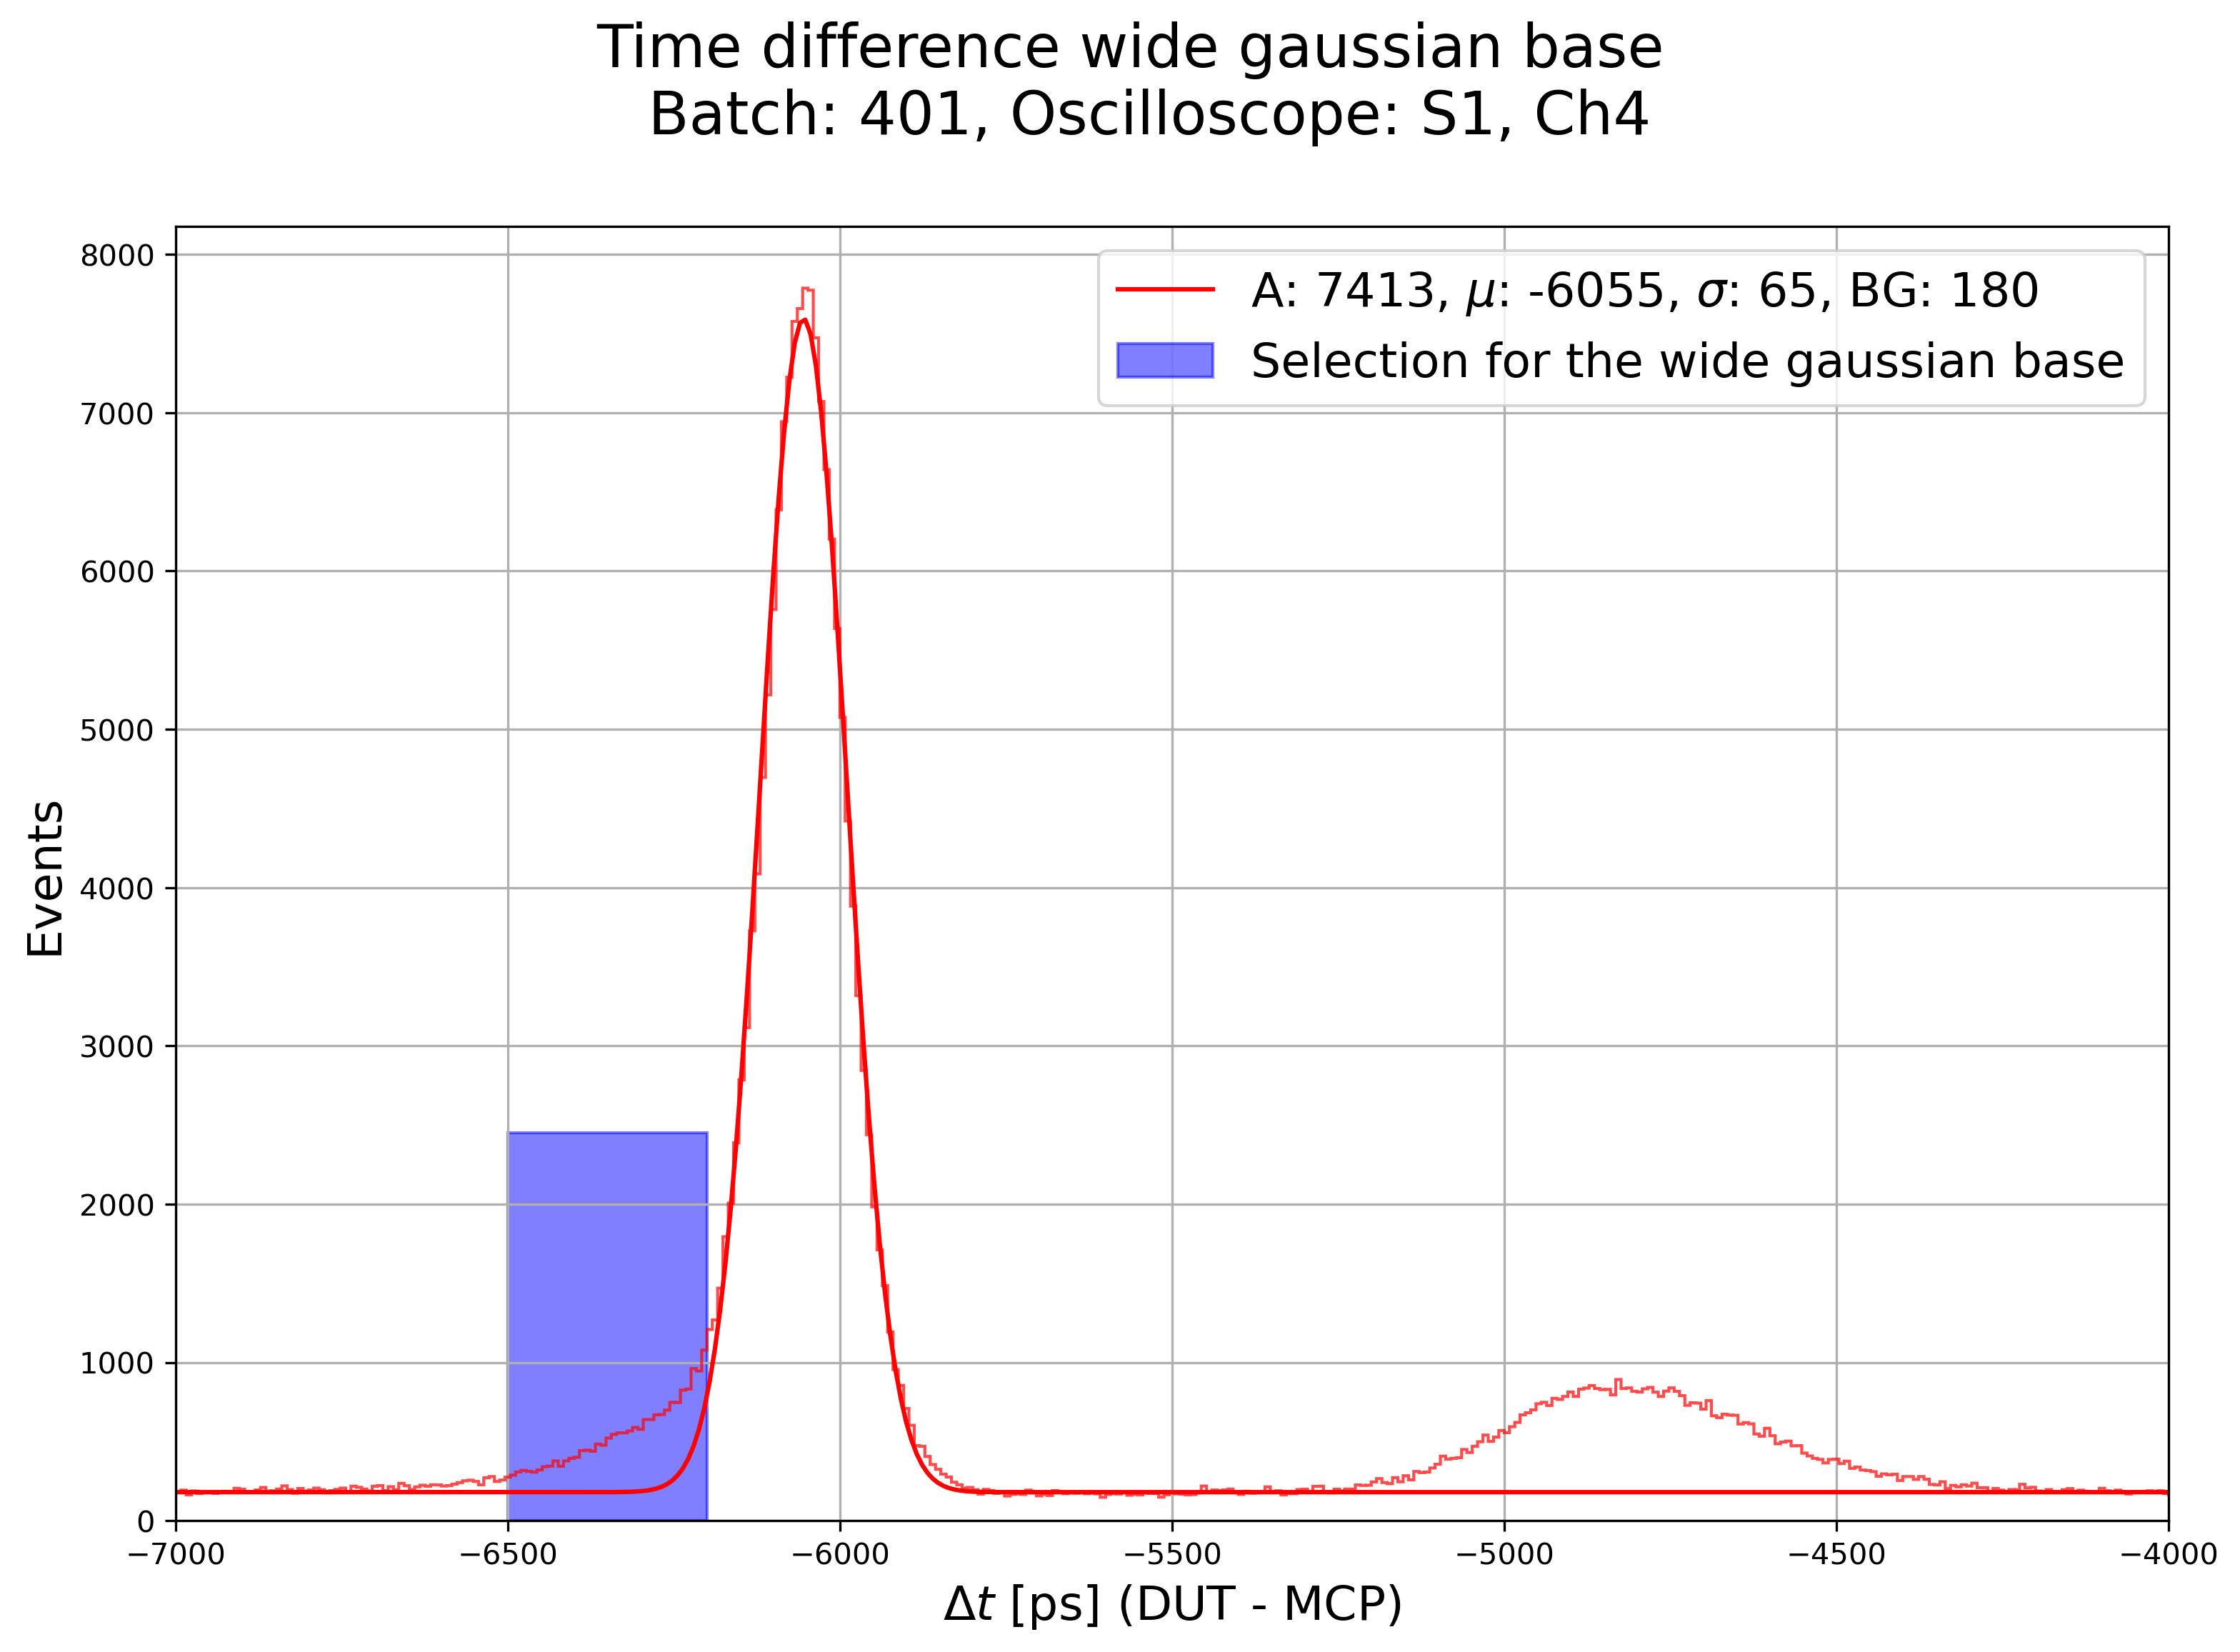
\includegraphics[width=.55\linewidth]{Images/detailed_analysis/time_difference_401_S1_dut_3_with_wide gaussian_left.png}}
    \hfill
    \subfloat[2D plot of the tracks inside the blue area, highlighting how they mostly originate from the edges of the sensor. The red rectangle outlined indicates the \textit{geometry cut}, for reference.]{
        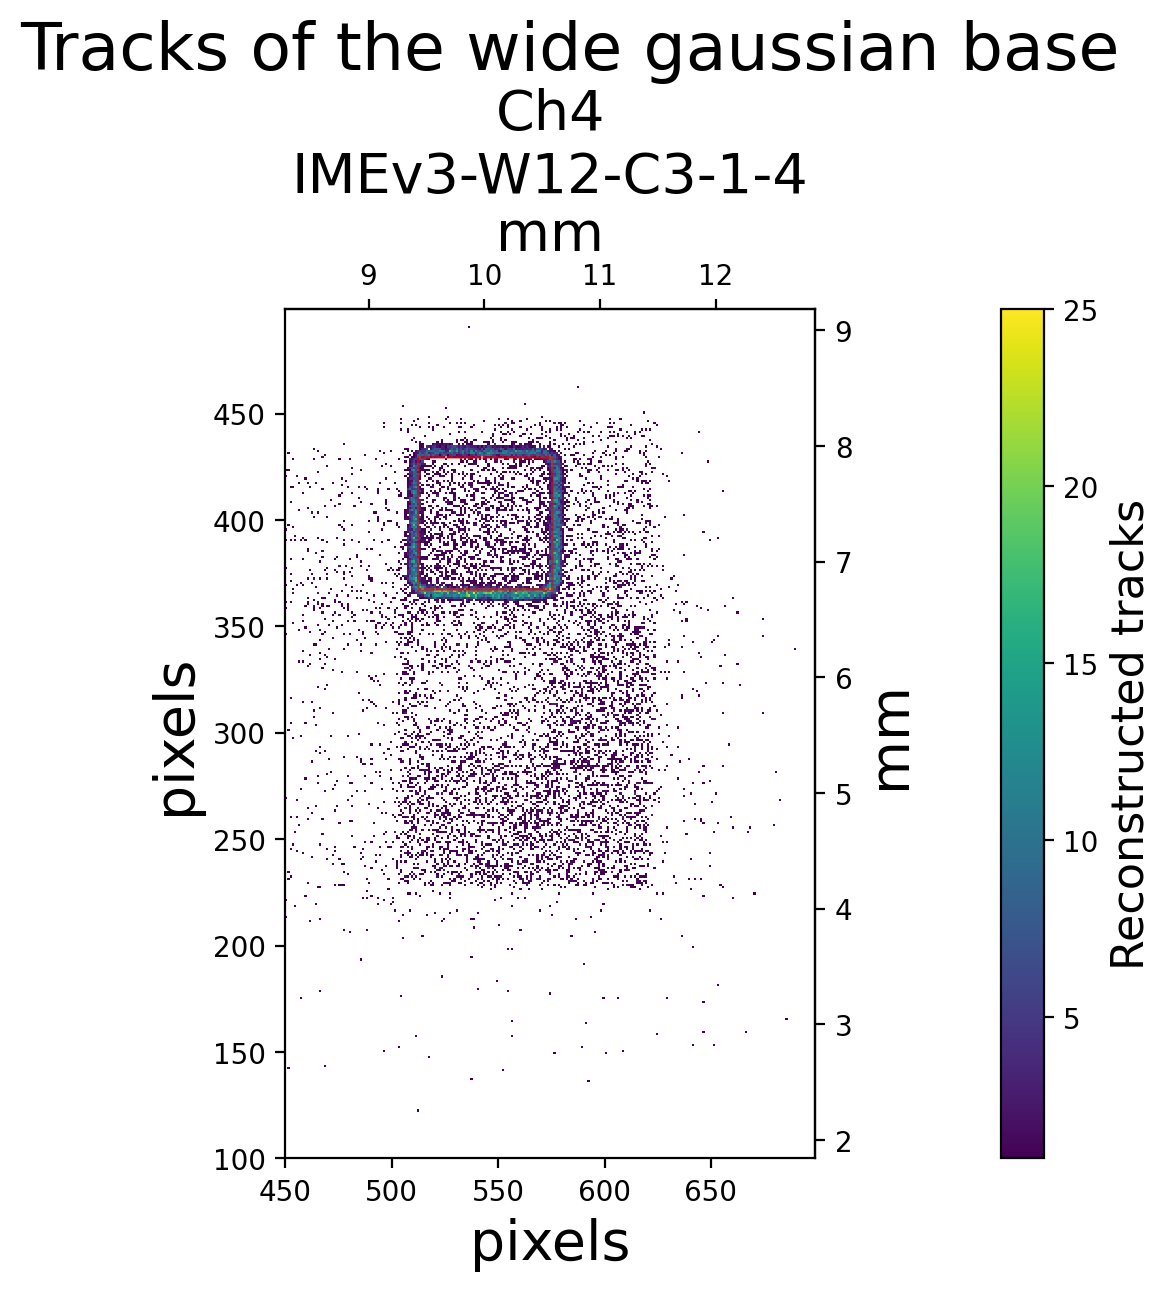
\includegraphics[width=.43\linewidth]{Images/detailed_analysis/2D Tracks 401_S1_dut_3_with_wide_gaussian_base_left.png}}
    \captionsetup{width=\captionwidth}
    \caption{Left: time distribution of the events, with the anomalous "wide base" in blue. \\
    Right: plot of all the tracks inside the blue interval.}
    \label{fig:time_difference_wide_gaussian}
\end{figure}


\subsection{Signal from neighbouring pads}\label{sec:multiple_peaks}

As the momentum of the incident particles was fixed, and the distance between the MCP and the DUTs was not changed during the runs, the time of flight from MCP to DUTs should peak at one point, not two, as shown in Figure~\ref{fig:time_cut_gauss+bg_fit}. 

The nature of the second peak was investigated by checking the spatial characteristics of the associated events, i.e. selecting all the events inside this time window and checking the spatial projection of the tracks on the DUT. It was found that the main peak simply coincides with the DUT, and the second peak arises from events picked up by its neighbouring pad. Figure~\ref{fig:time_difference_multiple_peaks_highlight} is evidence of this. This second group of events was observed with a delay of the order of \qty{1}{\nano\second}.
As further confirmation, this effect was only observed in DUTs which were part of LGAD arrays.

\begin{figure}[h!tbp]
    \centering
    \subfloat[Time distribution of the events, with the first and second peak highlighted in yellow and green, respectively.]{
        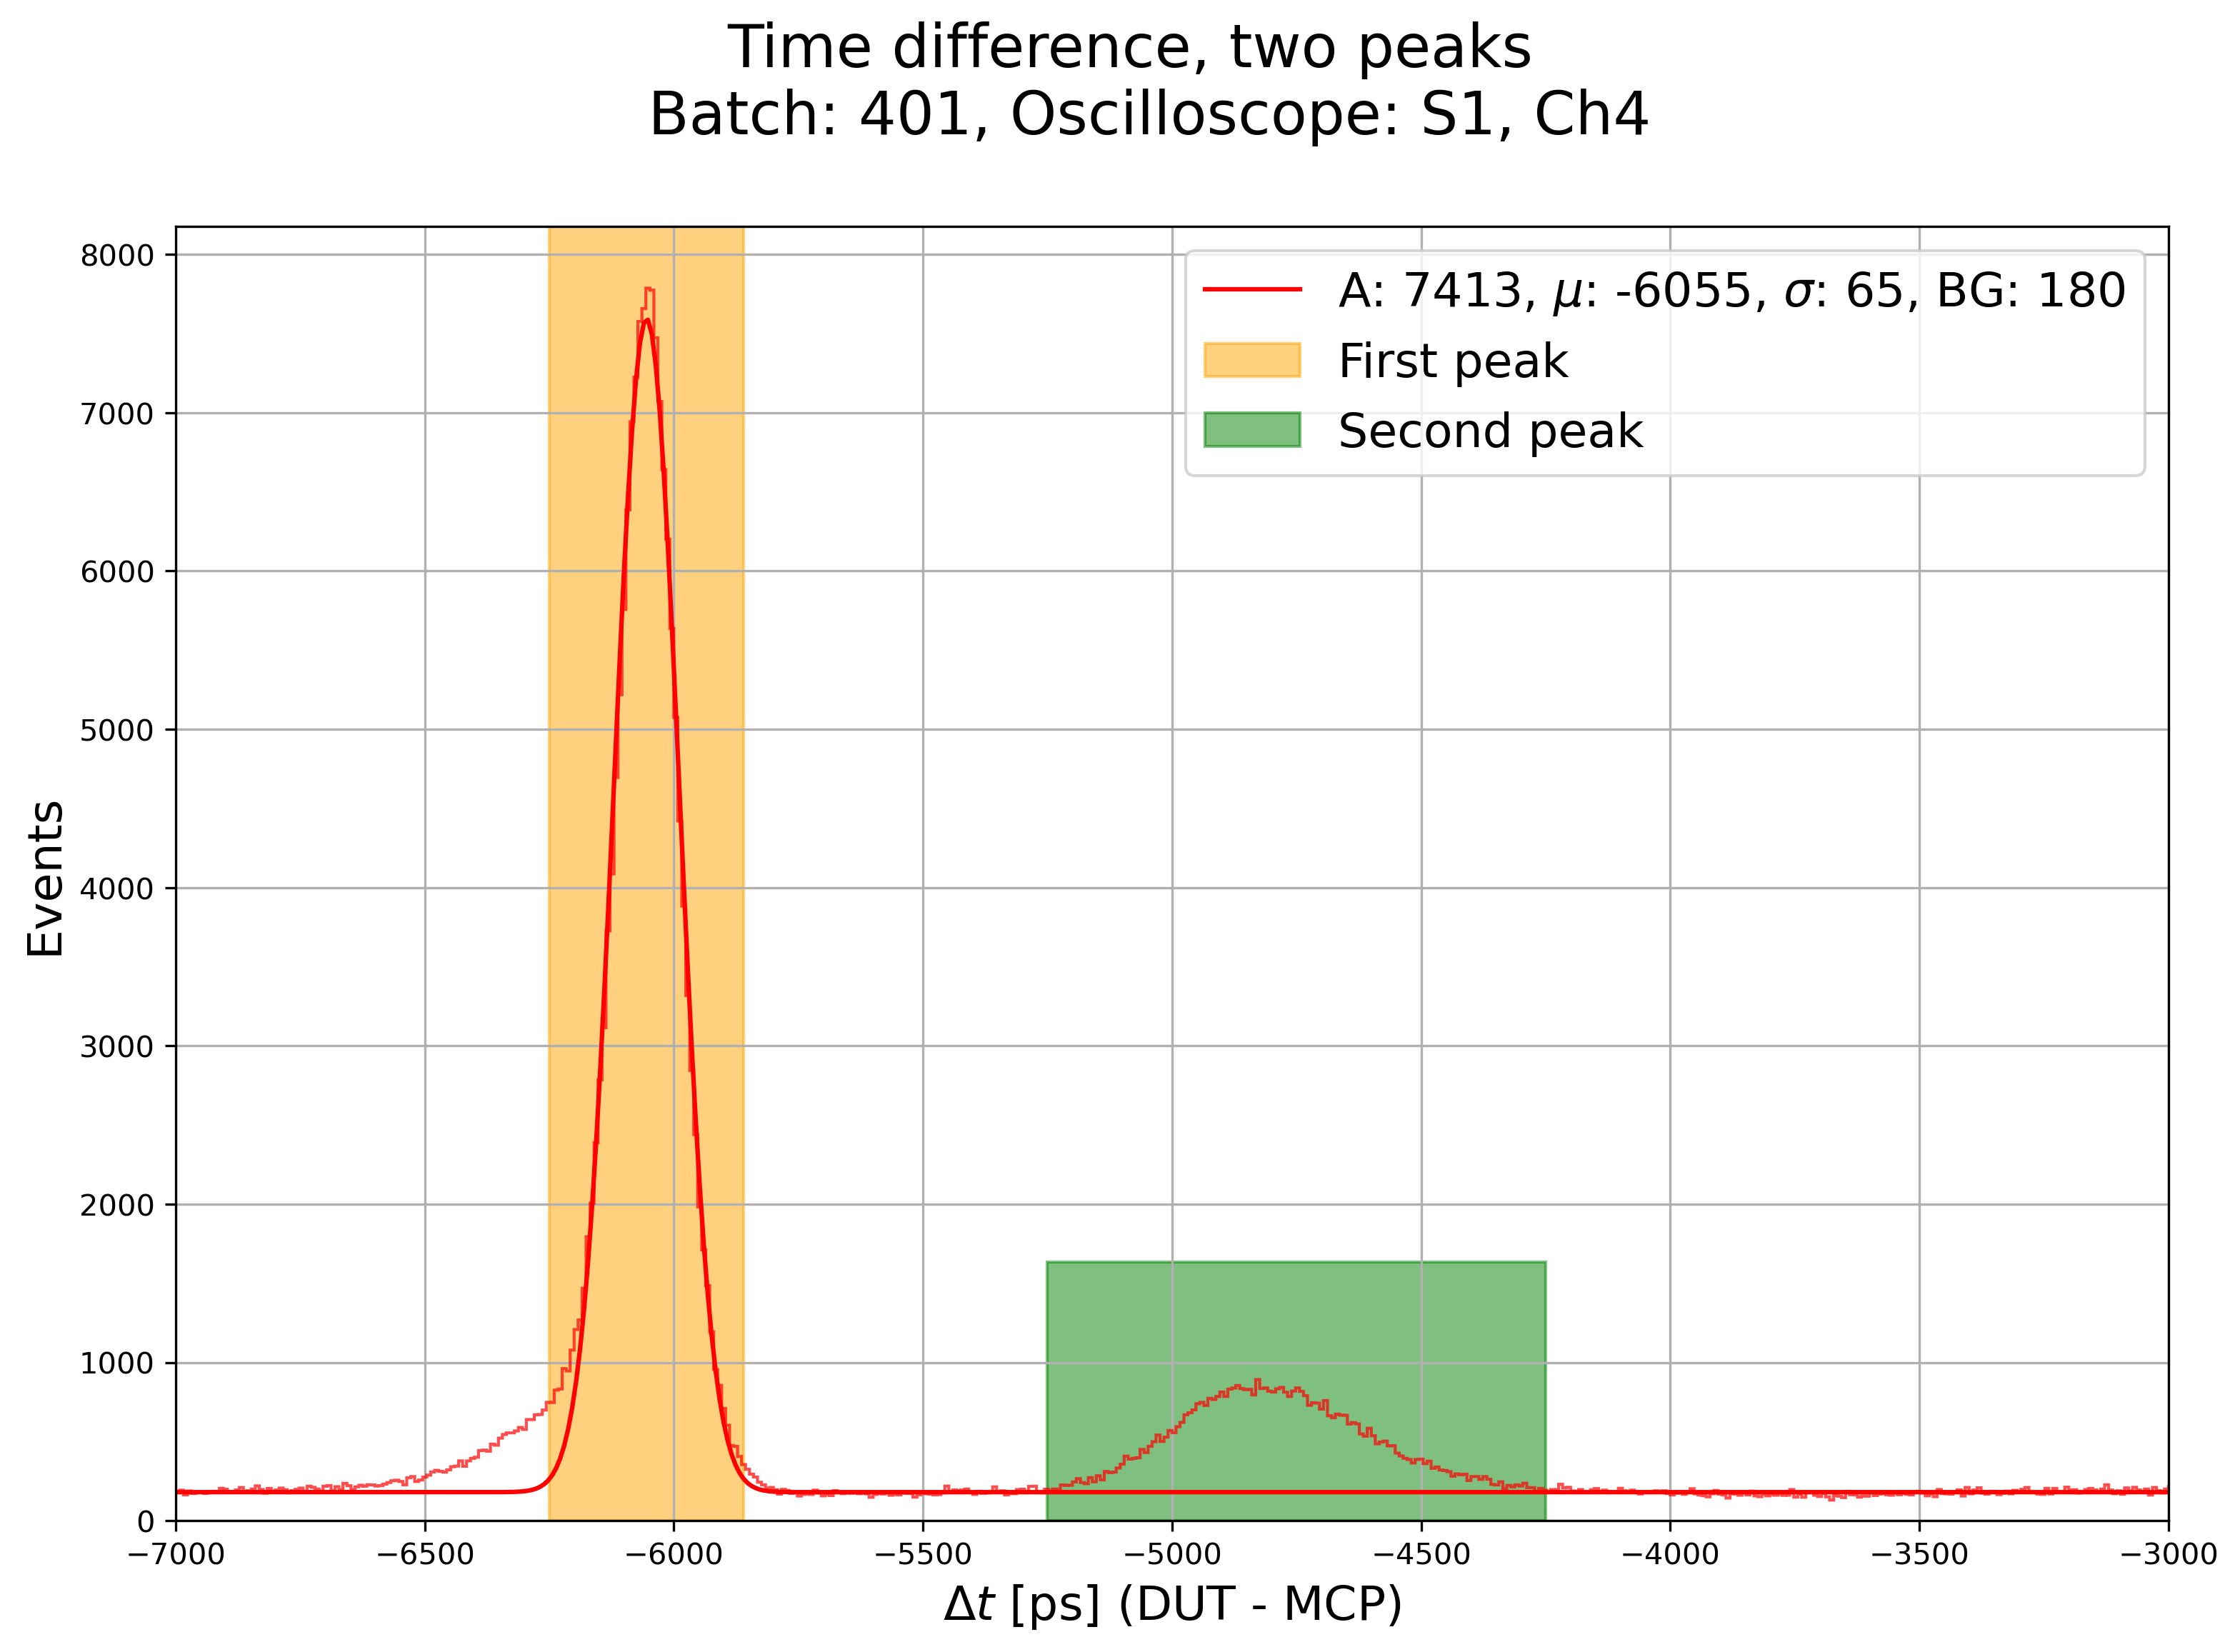
\includegraphics[width=.6\linewidth]{Images/detailed_analysis/time_difference_401_S1_dut_3_with_both_peaks_simple.png}}
    \\ [\smallskipamount]
    \subfloat[2D plot of the tracks inside the yellow first peak, revealing the connected pad]{
        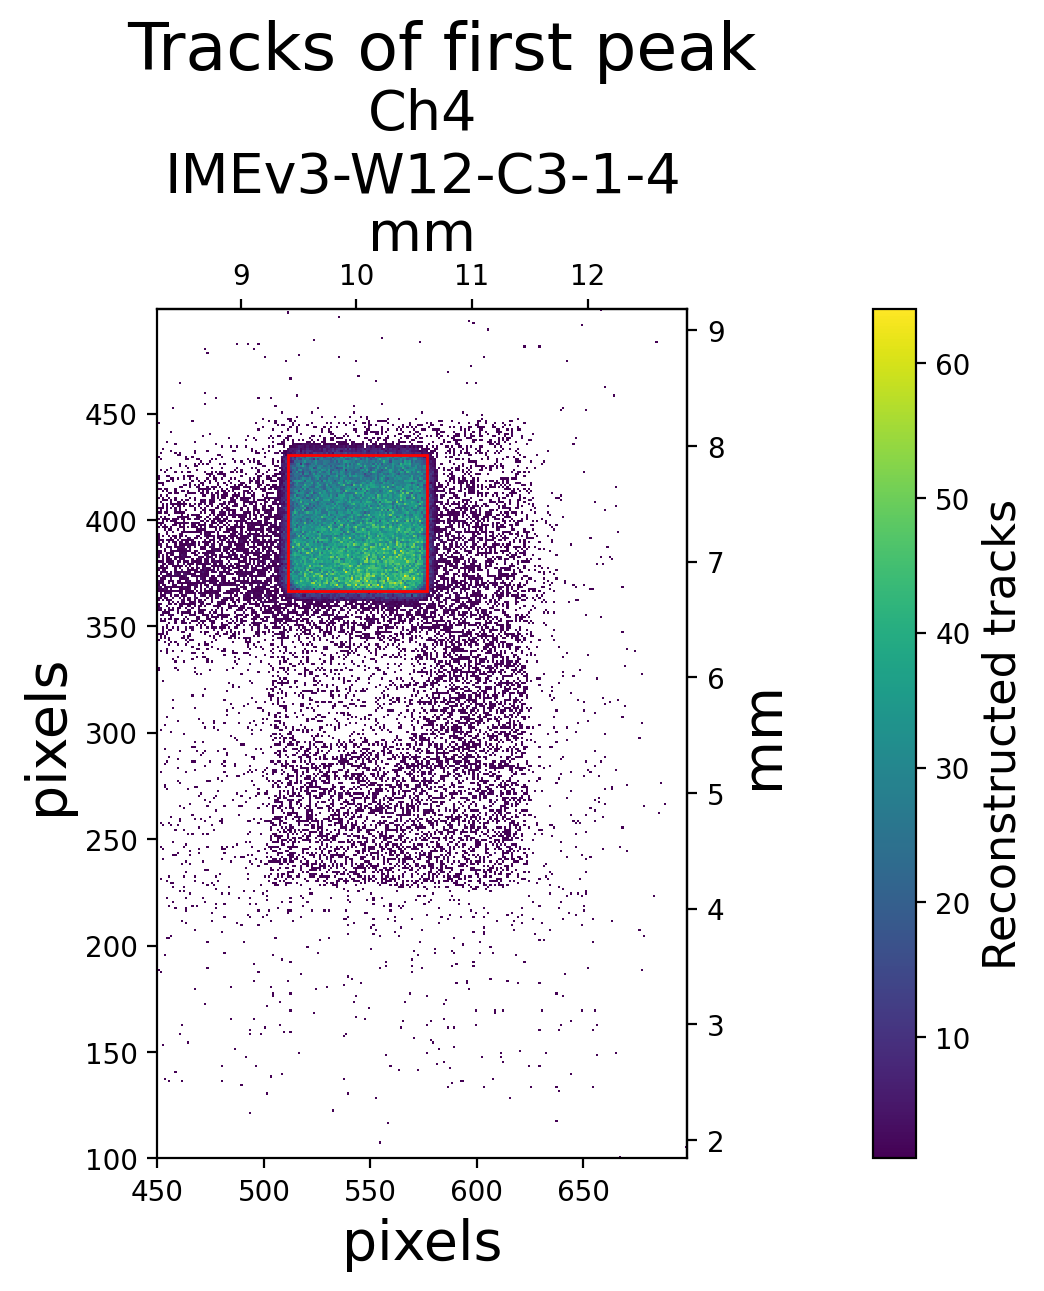
\includegraphics[width=.47\linewidth]{Images/detailed_analysis/2D Tracks 401_S1_dut_3_with_first_peak.png}}
    \hfill
    \subfloat[2D plot of the tracks inside the green second peak, revealing the connected pad]{
        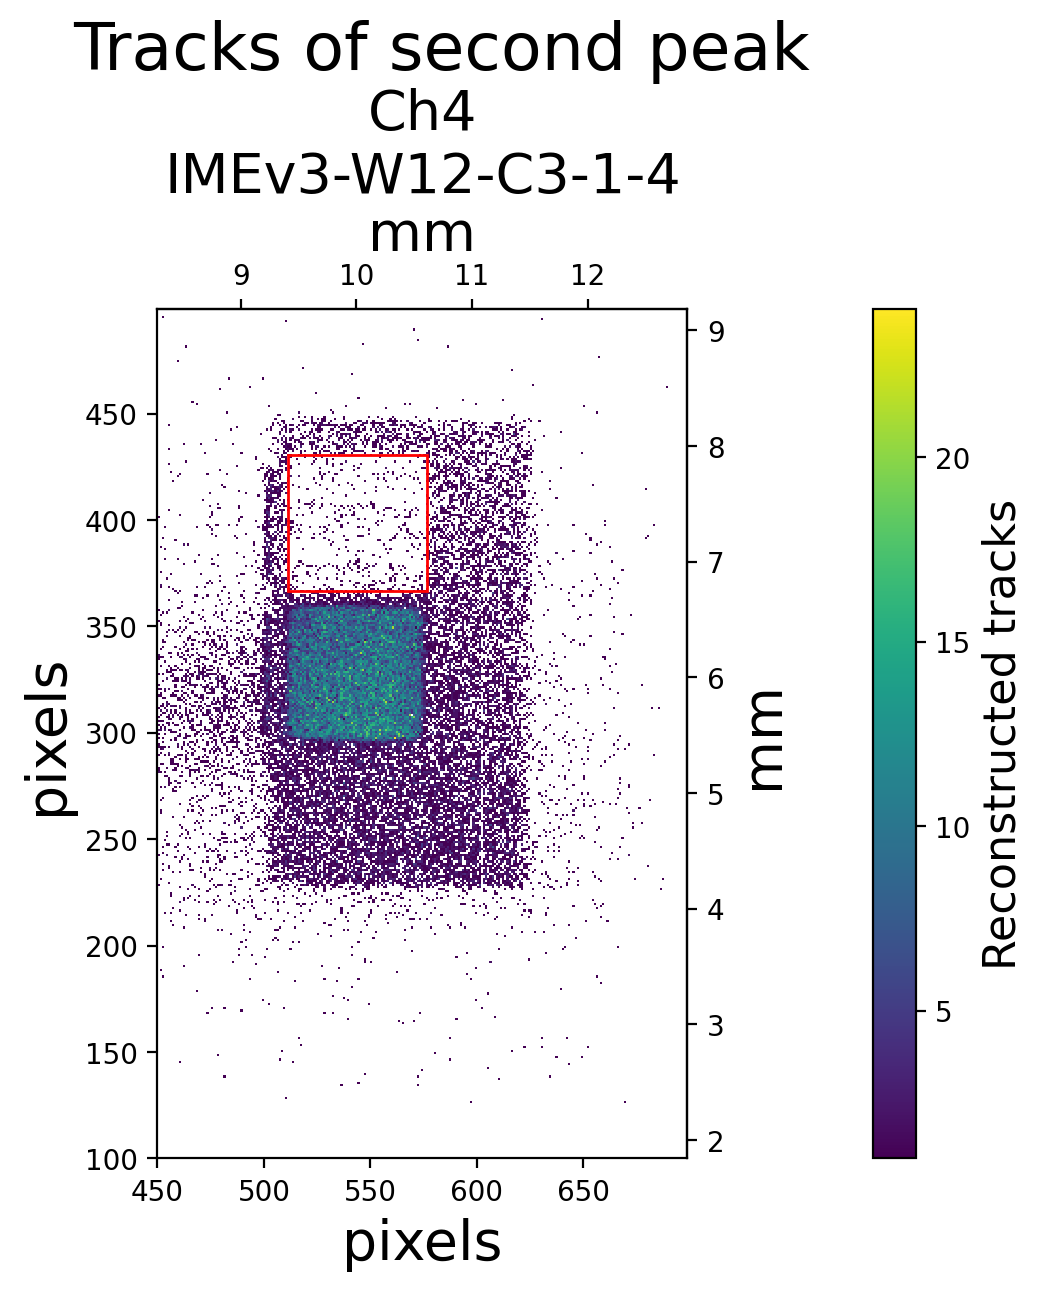
\includegraphics[width=.47\linewidth]{Images/detailed_analysis/2D Tracks 401_S1_dut_3_with_second_peak.png}}
    \captionsetup{width=\captionwidth}
    \caption{Top: Time difference (DUT-MCP) distribution, with the first and second peak highlighted.
    Left: Tracks of events inside the yellow interval. Right: Tracks of events inside the green interval. In red is the outline of the DUT, estimated with the \textit{geometry cut}.}
    \label{fig:time_difference_multiple_peaks_highlight}
\end{figure}

\FloatBarrier

\subsection{Pulse clipping}\label{sec:pulse_clipping}

As briefly mentioned before, there was indirect evidence that the pulses recorded by the oscilloscopes had been "cut" at their highest point. To verify this, the waveforms data was directly investigated, and a sample is shown in Figure~\ref{fig:clipped_pulse}. The apex of the pulse shows clearly a spurious plateau caused by the voltage value exceeding the range set on the oscilloscope. The consequences of this were:

\begin{itemize}
    \item Anomaly in the pulse height distribution (Figure~\ref{fig:pulseHeight_cut})
    \item Irregularities in the charge distribution (Figure~\ref{fig:charge_vs_pulseHeight_for_clipping})
\end{itemize}

Fortunately, this effect only impacted a small percentage of the data, thus it did not have a significant impact on the analysis.

\begin{figure}[h!tbp]
    \centering
    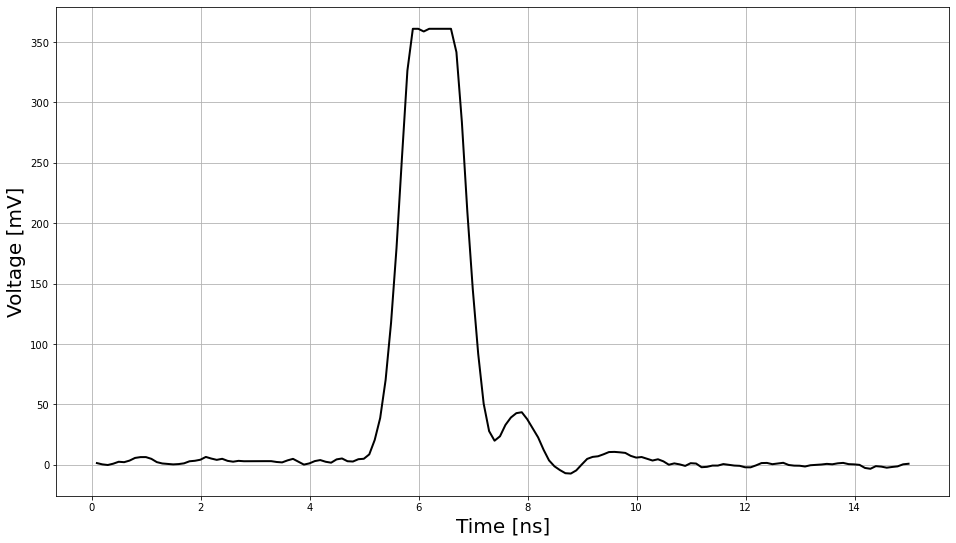
\includegraphics[width=.9\linewidth]{Images/detailed_analysis/Waveform of clipped pulse (ns).png}
    \captionsetup{width=\captionwidth}
    \caption{Example of a single pulse with the highest points cut out}
    \label{fig:clipped_pulse}
\end{figure}
 

\subsubsection{Irregularities in the charge distribution}\label{subsec:charge_irregularities}

In a few cases the tail portion of the charge distribution deviated considerably from the expected function, left graph of Figure~\ref{fig:charge_vs_pulseHeight_for_clipping}, as a consequence of the pulse clipping. In the right graph of Figure~\ref{fig:charge_vs_pulseHeight_for_clipping} the pulse height is plotted against the charge and the clipped events appear distinctly at the rightmost part of the plot. This group of events overlapped with the expected charge distribution and could not be removed without altering it. For this reason, the only solution was to adjust the range of the fit to exclude these events.

\begin{figure}[h!tbp]
    \centering
    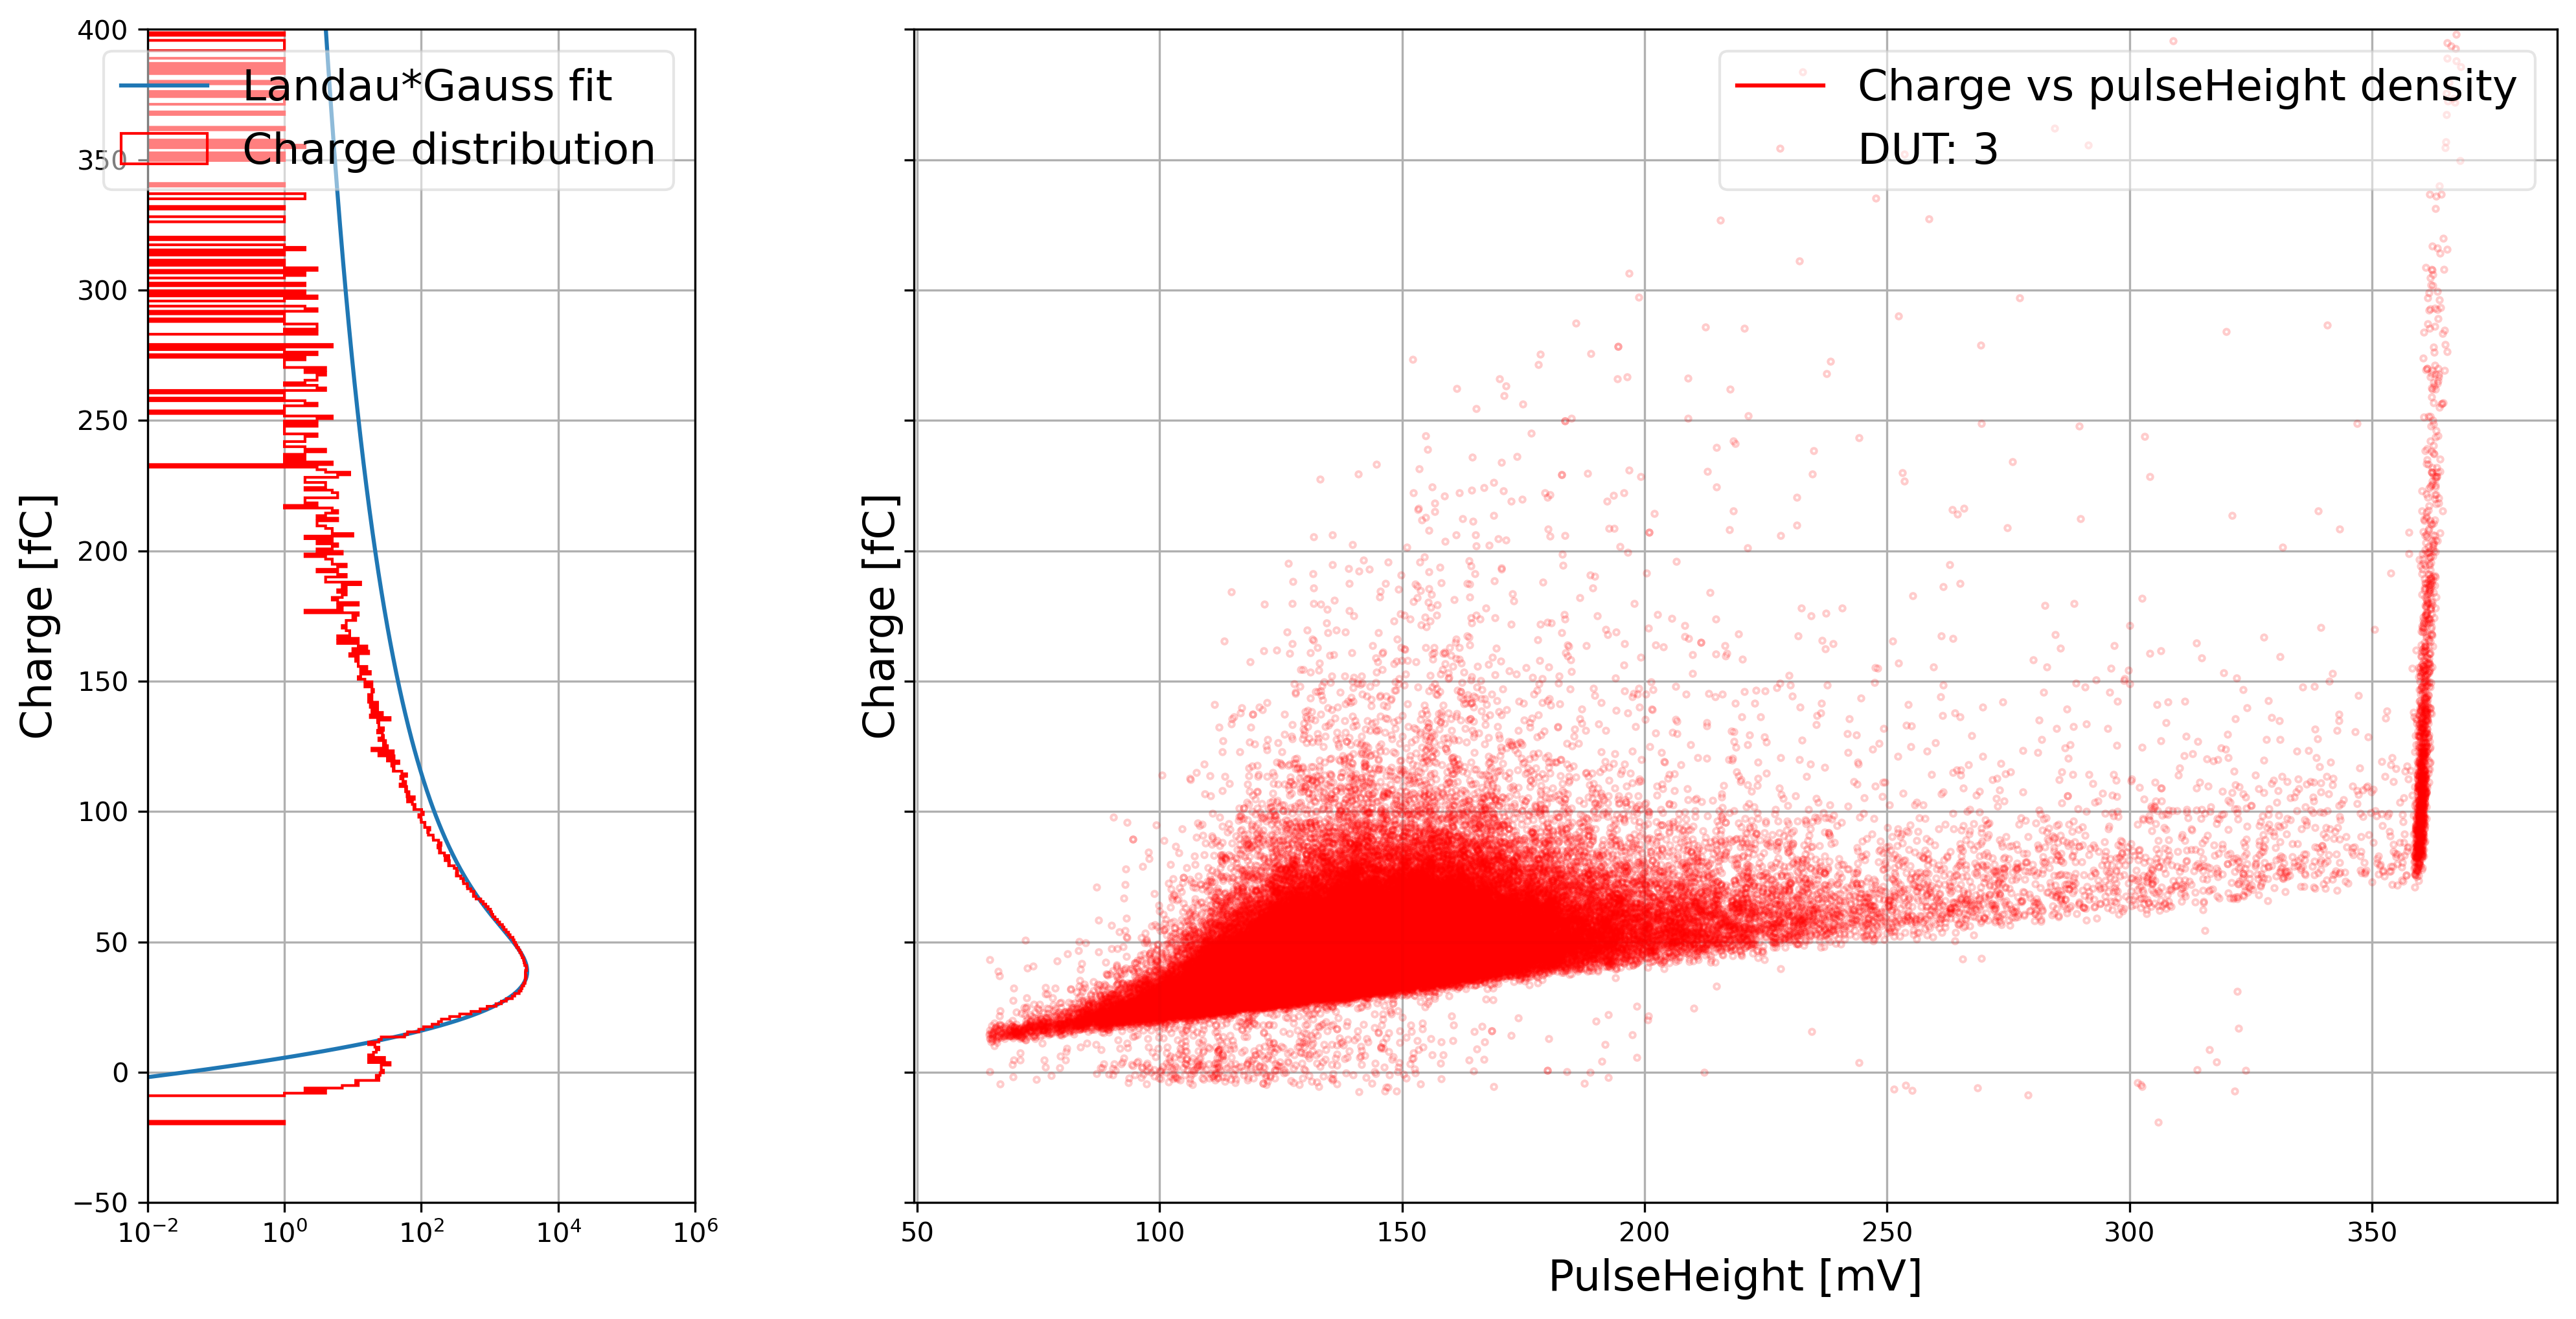
\includegraphics[width=1\linewidth]{Images/detailed_analysis/Charge_vs_pulseHeight_density_413_S2_dut3.png}
    \captionsetup{width=\captionwidth}
    \caption{Left: distribution of collected charge with Gaussian*Landau fit, the tail shows a significant deviation between fit and data. \\
    Right: scatter plot of Pulse height vs Charge, revealing a dense line of events with identical pulse height, caused by the clipping.}
    \label{fig:charge_vs_pulseHeight_for_clipping}
\end{figure}

\FloatBarrier

\subsection{Temperature fluctuations}\label{sec:temperature_fluctuations}

During the data taking there was a short malfunction of the cooling box containing the DUTs, which caused the temperature to rise up to \(\approx\qty{-26}{\degreeCelsius}\). The  batch was excluded from the previous analysis, but it showed that the sensors have a significant sensitivity to temperature, so it was deemed interesting enough to report. For a change in temperature of \(\approx\qty{6}{\degreeCelsius}\), the collected charge saw a decrease of up to \(\approx\qty{10}{\femto\coulomb}\) and time resolution saw a decrease of up to \(\approx\qty{3}{\pico\second}\).

\begin{figure}[h!tbp]
    \centering
    \begin{minipage}[c]{.49\linewidth}
        \subfloat[Temperature vs Charge, DUTs on oscilloscope 1]{
            \includegraphics[width=.95\linewidth]{Images/Results/temperature fluctuations/Charge vs temperature 413_S1_dut[1, 2, 3].png}
            \label{fig:temperature_charge_S1}}
        \end{minipage}
        \hfill
        \begin{minipage}[c]{.49\linewidth}
        \subfloat[Temperature vs Time resolution, DUTs on oscilloscope 1]{
            \includegraphics[width=.95\linewidth]{Images/Results/temperature fluctuations/Time resolution vs temperature 413_S1_dut[1, 2, 3].png}
        \label{fig:temperature_time_res_S1}}
    \end{minipage}
    \vfill
    \begin{minipage}[c]{.49\linewidth}
        \subfloat[Temperature vs Charge, DUTs on oscilloscope 2]{
            \includegraphics[width=.95\linewidth]{Images/Results/temperature fluctuations/Charge vs temperature 413_S2_dut[1, 2, 3].png}
            \label{fig:temperature_charge_S2}}
        \end{minipage}
        \hfill
        \begin{minipage}[c]{.49\linewidth}
        \subfloat[Temperature vs Time resolution, DUTs on oscilloscope 2]{
            \includegraphics[width=.95\linewidth]{Images/Results/temperature fluctuations/Time resolution vs temperature 413_S2_dut[1, 2, 3].png}
            \label{fig:temperature_time_res_S2}}
        \end{minipage}
    
    \captionsetup{width=\captionwidth}
    \caption{Plots of the charge and the time resolution as function of the temperature, showing a clear dependence across all sensors. NB: The sensors shown here were operated at different voltages, so this plot is not meant to be a comparison between them, rather an observation of the general trend of each of them individually.}
\end{figure}

\FloatBarrier
\subsection{Interpad study}\label{sec:neighbouring_pads}
%%% TODO: put more plots and description? tbh I don't know what would the conclusions be

The following plots show the efficiency of the interpad region, as a function of the position. The location data was projected onto the X axis (Y axis) and, for each bin, the efficiency was calculated in a vertical (horizontal) strip. The analysis of the IMEv3-W12-2x2 was discarded due a small but significant tilt of the sensor in the XY plane (Figure~\ref{fig:tilted_sensors}). This inclination meant that the projections of the positions onto one axis would not be well aligned. 

%%% IMEv3-W12-1x3
\begin{figure}[h!tbp]
    \centering
    \subfloat[Interpad efficiency, \qty{80}{\volt}]{
        \includegraphics[width=.3\linewidth]{Images/detailed_analysis/interpad studies/1D_Efficiency_on_the_edges_IMEv3-W12-1x3_401_-80V_duts_3_3.png}
        \label{fig:IMEv3-W12-1x3_interpad_80V}}
    \hfill
    \subfloat[Interpad efficiency, \qty{90}{\volt}]{
        \includegraphics[width=.3\linewidth]{Images/detailed_analysis/interpad studies/1D_Efficiency_on_the_edges_IMEv3-W12-1x3_402_-90V_duts_3_3.png}
        \label{fig:IMEv3-W12-1x3_interpad_90V}}
    \hfill
    \subfloat[Interpad efficiency, \qty{100}{\volt}]{
        \includegraphics[width=.3\linewidth]{Images/detailed_analysis/interpad studies/1D_Efficiency_on_the_edges_IMEv3-W12-1x3_403_-100V_duts_3_3.png}
        \label{fig:IMEv3-W12-1x3_interpad_100V}}
    \vfill

    \begin{minipage}[c]{.31\linewidth}
        \subfloat[Interpad efficiency, \qty{125}{\volt}]{
            \includegraphics[width=.95\linewidth]{Images/detailed_analysis/interpad studies/1D_Efficiency_on_the_edges_IMEv3-W12-1x3_407_-125V_duts_3_3.png}
            \label{fig:IMEv3-W12-1x3_interpad_125V}}
        \end{minipage}
        \hfill
    \begin{minipage}[c]{.65\linewidth}
        \captionof{figure}{For the unirradiated IME sensor, the pads had a fairly narrow region of low efficiency, with a valley at \(\approx 10\%\) efficiency, which remained mostly stable from \qtyrange{-90}{-125}{\volt}.}
    \end{minipage}
\end{figure}

%%% IMEv3-W12-2x2-1.5E15
\begin{figure}[h!tbp]
    \centering
    \subfloat[Interpad efficiency, \qty{300}{\volt}]{
        \includegraphics[width=.3\linewidth]{Images/detailed_analysis/interpad studies/1D_Efficiency_on_the_edges_IMEv3-W12-2x2-1.5E15_601_-300V_duts_1_2.png}
        \label{fig:IMEv3-W12-2x2_interpad_300V}}
    \hfill
    \subfloat[Interpad efficiency, \qty{350}{\volt}]{
        \includegraphics[width=.3\linewidth]{Images/detailed_analysis/interpad studies/1D_Efficiency_on_the_edges_IMEv3-W12-2x2-1.5E15_602_-350V_duts_1_2.png}
        \label{fig:IMEv3-W12-2x2_interpad_350V}}
    \hfill
    \subfloat[Interpad efficiency, \qty{400}{\volt}]{
        \includegraphics[width=.3\linewidth]{Images/detailed_analysis/interpad studies/1D_Efficiency_on_the_edges_IMEv3-W12-2x2-1.5E15_603_-400V_duts_1_2.png}
        \label{fig:IMEv3-W12-2x2_interpad_400V}}
    \vfill

    \begin{minipage}[c]{.62\linewidth}
        \subfloat[Interpad efficiency, \qty{450}{\volt}]{
            \includegraphics[width=.47\linewidth]{Images/detailed_analysis/interpad studies/1D_Efficiency_on_the_edges_IMEv3-W12-2x2-1.5E15_604_-450V_duts_1_2.png}
            \label{fig:IMEv3-W12-2x2_interpad_450V}}
        \hfill
        \subfloat[Interpad efficiency, \qty{490}{\volt}]{
            \includegraphics[width=.47\linewidth]{Images/detailed_analysis/interpad studies/1D_Efficiency_on_the_edges_IMEv3-W12-2x2-1.5E15_605_-490V_duts_1_2.png}
            \label{fig:IMEv3-W12-2x2_interpad_490V}}
        \end{minipage}
        \hfill
    \begin{minipage}[c]{.31\linewidth}
        \captionof{figure}{The sensor IMEv3-W12-2x2-1.5E15 showed a significant improvement of the lowest efficiency in the gap, especially above \qty{-490}{\volt}. The regularly spaced dips in efficiency, may have been caused by some physical element interfering with the beam, as this effect was observed in many sensors.}
    \end{minipage}
\end{figure}


%%% USTC
\begin{figure}[h!tbp]
    \centering
    \subfloat[Interpad efficiency, \qty{80}{\volt}]{
        \includegraphics[width=.3\linewidth]{Images/detailed_analysis/interpad studies/1D_Efficiency_on_the_edges_USTC2.1-W17_401_-80V_duts_1_2.png}
        \label{fig:USTC2.1-W17_interpad_80V}}
    \hfill
    \subfloat[Interpad efficiency, \qty{90}{\volt}]{
        \includegraphics[width=.3\linewidth]{Images/detailed_analysis/interpad studies/1D_Efficiency_on_the_edges_USTC2.1-W17_402_-90V_duts_1_2.png}
        \label{fig:USTC2.1-W17_interpad_90V}}
    \hfill
    \subfloat[Interpad efficiency, \qty{100}{\volt}]{
        \includegraphics[width=.3\linewidth]{Images/detailed_analysis/interpad studies/1D_Efficiency_on_the_edges_USTC2.1-W17_403_-100V_duts_1_2.png}
        \label{fig:USTC2.1-W17_interpad_100V}}
    \vfill

    \begin{minipage}[c]{.31\linewidth}
        \subfloat[Interpad efficiency, \qty{105}{\volt}]{
            \includegraphics[width=.95\linewidth]{Images/detailed_analysis/interpad studies/1D_Efficiency_on_the_edges_USTC2.1-W17_407_-105V_duts_1_2.png}
            \label{fig:USTC2.1-W17_interpad_105V}}
        \end{minipage}
        \hfill
    \begin{minipage}[c]{.65\linewidth}
        \captionof{figure}{The sensor USTC2.1-W17 displayed very little change in the interpad region, with the width and depth of the gap staying mostly constant from \qtyrange{-80}{-105}{\volt}.}
    \end{minipage}
\end{figure}


% \begin{figure}[h!tbp]
%     \centering
%     \includegraphics[width=0.5\linewidth]{Images/detailed_analysis/interpad studies/}
%     \captionsetup{width=\captionwidth}
%     \caption{Efficiency projected onto one direction, measured between two neighbouring pads.}
%     \label{fig:neighbouring_pads}
% \end{figure}

